\documentclass[a4paper,12pt]{article}

% AMS packages:
\usepackage{amsmath, amsthm, amsfonts}
\usepackage{graphicx}

\providecommand{\keywords}[1]{\textbf{\textit{Keywords:}} #1}

%-----------------------------------------------------------------
\title
{
	UNSUPERVISED MACHINE TRANSLATION USING MONOLINGUAL CORPORA ONLY
}



\author
{
	Omar Faruk Riyad  \\
	1610634042 \\ 
	North South University  \\
	\and 
	Arif Suhan \\
	1610437042 \\
	North South University  \\
}

\begin{document}
\maketitle

\abstract
{
	Machine translation has recently achieved impressive performance thanks to recent advances in deep learning and the availability of large-scale parallel corpora. There have been numerous attempts to extend these successes to low-resource language pairs, yet requiring tens of thousands of parallel sentences. In this work, we take this research direction to the extreme and investigate whether it is possible to learn to translate even without any parallel data. We propose a model that takes sentences from monolingual corpora in two different languages and maps them into the same latent space. By learning to reconstruct in both languages from this shared feature space, the model effectively learns to translate without using any labeled data. We demonstrate our model on two widely used datasets and two language pairs, reporting BLEU scores of 32.8 and 15.1 on the Multi30k and WMT English-Bengali datasets, without using even a single parallel sentence at training time.\cite{ref1}
} 

% \keywords{ideal of sets; nowhere dense; analytic}

\section{Introduction}

Since the dawn of the internet, reducing network load while transferring data has been the great challenge of computer science. As the most transferred data over the network are image data, if we could get high-resolution images from the low resolution that could save the network load by a significant amount. We wanted to try out a working mechanism that could achieve this particular goal while leaving the heavy duty on the user's computer. The state-of-the-art architecture ProSR is one of the best ways to retain image information to convert a low-resolution image to high resolution. The mechanism that we tried was to perform the computation on the browser side. While the data sent by the server is low-resolution image later it will be generated as high resolution. To make a dense model work in the browser is a challenging task. Along with the dense layer they have also used bicubic interpolation layer by layer to make the high resolution even better for this particular model. The sole purpose of choosing a complex network is exploration the compatibility issues over variations of interfaces, in this case, pure JavaScript without any libraries.

Reducing network load while transfering data has been the great challenge of computer science since the dawn of the internet. Since the most transferred data over the network are image data, if we could get high resolution images from low resolution could save the network load by significant amount. We wanted to try out a working mechanism that could achieve this particular goal while leaving the heavy duty on the user's computer. The state-of - the-art architecture ProSR is one of the best ways to retain image information to convert a low resolutionresolution image to high resolution. The mechanism that we tried was to perform the computation on the browser side. while the data sent by the server is low resolution image later it will be generated as high resolution. To make a dense model to work in the browser is a challenging task. Along with the dense layer they have also used bicubic interpolation layer by layer to make the high resolution even better for this particular model. The sole purpose of chosing a complex network is exploration the compatebility issues over variations of interfaces, in this case pure JavaScript without any libraries.


\section{Model Description}

\subsection{DenseNet}
Dense networks are the next step in increasing the profundities of deep convolutional networks. When CNNs go deeper, the problems arise. This is because the path from the input layer for information becomes so large that it can disappear before reaching the other part of the output layer (and the gradient is in the opposite direction). DenseNets simplify the pattern of connectivity among layers in other architectures. 

\subsection{ProSR GAN}
Generative adversarial networks (GANs) have emerged as a powerful method to enhance the perceptual quality of the upsampled images in SISR.The model ProSR contained a dense layer and a dense compression unit. The model also used bicubic interpolation and addition with some of the layer output, for which it is one of the expensive model to perform computation with. But the result produced by this ProSR is amazing interms of quality of produced the image.
\cite{ref1}
\\
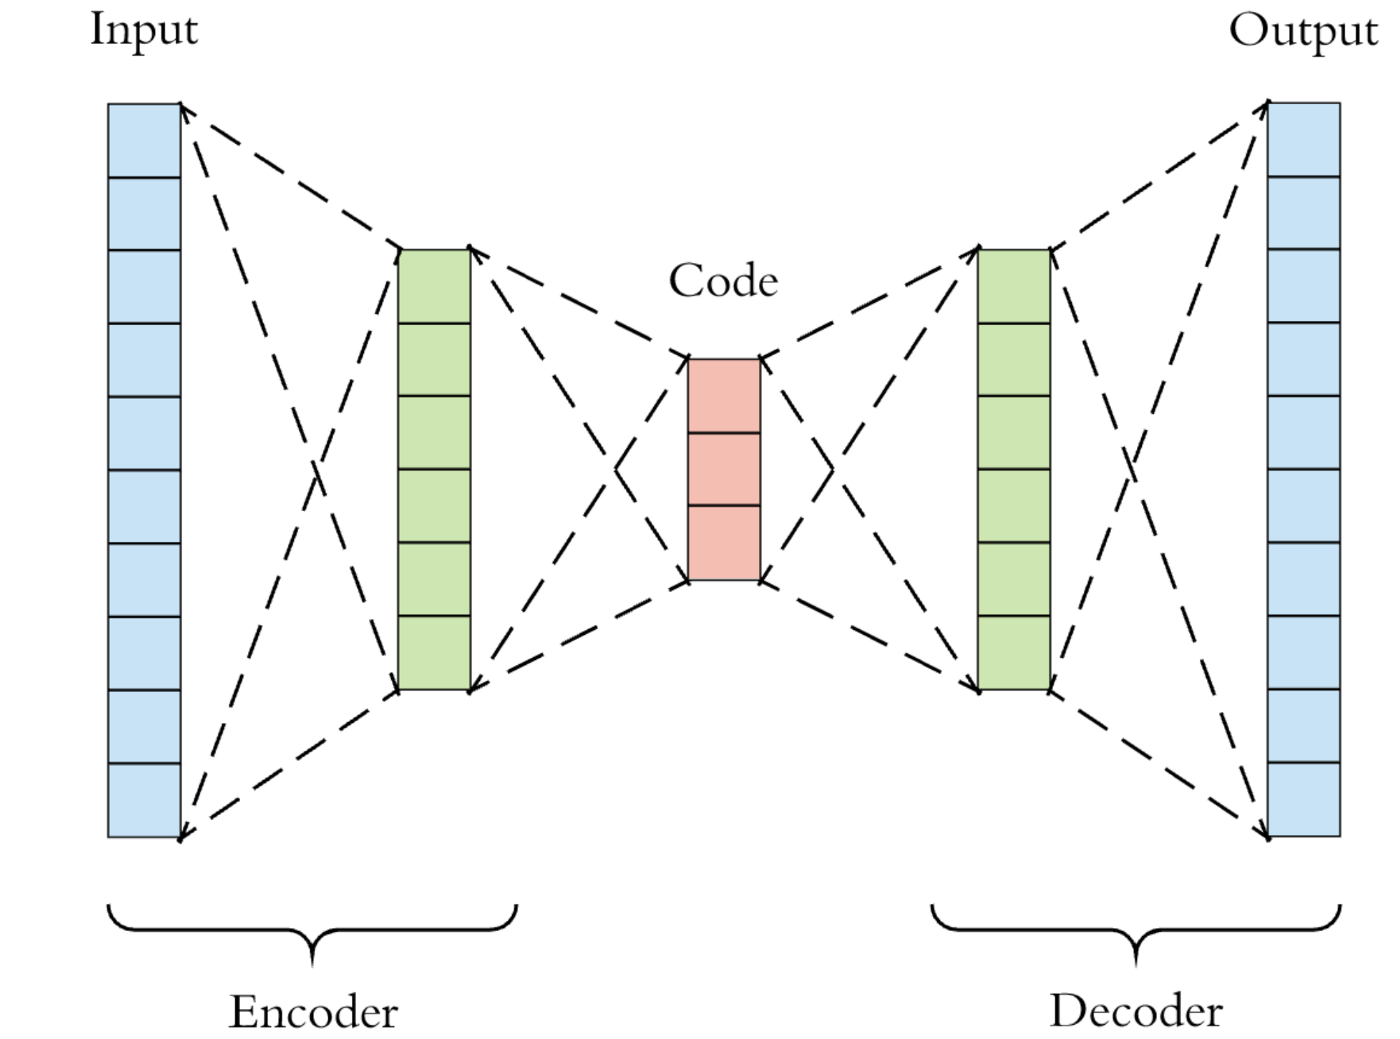
\includegraphics[width=\linewidth]{autoencoder.png}

\section{Challenges}

\subsection{Converting Model}

The first problem we got in order to get further with the idea is to convert the model to JavaScript natively. We tried out a bunch of different methods to convert the model but because of the model contained dense layer, it was really difficult to put into code since the sequence of the network has to be followed. We found that we could easily convert PyTorch model into an Open Neural Network Exchange (ONNX) model, from the base of ONNX it performs operations in Pure Basic Language. We extracted the Pure Basic Model code from the ONNX model, from which we found the underlying repeated network in the right sequence of its weights. We also found that there are 610 layers in the neural network and has about 7 operations which also have multiple different parameters. The pure Basic language is similar to native JavaScript, by performing some regex operation the code, we easily converted it to a native JavaScript code. 

This was the easiest challenges that we had to face over the entire time working with this project.

\subsection{Weight to JSON}
The next challenge that we had to face is to convert weights and load it to the browser. Converting the model weights to JSON was complex but it was easily done. Here again, we used the ONNX model to get the weights from since our model network was generated from the same model. The model had all weights in the sequence that we needed it to be thus parsing the weights wasn't difficult. At first, we worked with float32 data to have better precisions but the loading time was taking more than what we expected. Also, the file size has gotten about 345MB even after minifying the JSON file. It was a challenge to fix because we had to lower the file size and make it work at the same time because the browser couldn't cope up with the file. We solved this issue by reducing the weights from float32 to float16 which required fewer data and less memory size. It was not an easy thing to do but we had to choose float16 because of our operations were running in the CPU. We made work on the cost of losing precisions.

\subsection{Engine Compatibility}
At first, we were using Google Chrome to run our tests. But Google chrome runs on the chromev8 engine which we couldn't make it load the weights JSON faster. On the other hand, the firefox uses spidermonkey engine that makes faster to load the weights. Also most of the time, Google Chrome used to crush where firefox didn't.In the comparison of javascript engine compatibility, spidermonkey is better than chromev8 especially for loading JSON and garbage collection purpose.
As Spidermonkey compiles any javascript code to bytecode, it has an auto garbage collector. But chromev8 hasn't and it compiles the code to machine code.


\subsection{Performing Operations Issue }
Most of the users of the browser does not have GPU support since the whole idea of exploration was CPU based. Our JavaScript engine compiles the javascript code to byte code rather than machine code. So we lose some of the performance because of it. 

\subsection{Computation Issue}
Computation with the model was higher than we expected. Since it had a huge amount of weight and layers to it and the model used bicubic and previous layer output farther down the network. It had to store a lot of data to the memory. We tried some of the low-resolution images to convert them to high resolution but we failed. Also to finish computing of the full network model,
we need a lot of time for execution.


\section{What to expect}
If we could solve all these problems, we could have faster data transmission for which the network could be reduced to more than 25\% by assumption. This method is new and diversified to our current standards. We didn't tired training on JavaScript natively because that wasn't our sole purpose. But if we tried to write the model and retrain it we could achieve better result. However, that is out of the scope of what we were trying to achieve.

\section{Evalution}
\subsection{Run Time}
We run our model regarding other errors on the Firefox engine to see if it perform anyhow. But on runtime, we have seen that the model proSR usage 28GB of memory to perform computation, which is beyond anyone would expect. If we could maintain the memory better way we could achieve a bit better performance.

\section{Conclusion}
 In our exploration, we have seen that computing in the browser is highly costly to run operation. With an efficient library, we hope this problem can be solved. Also if we can use GPU for computing through the browser, the performance with increase a lot and save our time but most of the users don't have a GPU to begin with. Finally, it can be said that the idea of using deep learning in the browser could open up new opportunities in the realm of computer vision problems. 

The first problem we got in order to get farther with the idea is to convert the model to JavaScript natively. We tried out a bunch of different method to convert the model but because of the model contained dense layer, it was really difficult to put into code since the sequence of the network has to be followed. We found that we could easily convert PyTorch model into a  Open Neural Network Exchange (ONNX) model, from the base of ONNX it performs operations in Pure Basic Language. We extracted the Pure Basic Model code from the ONNX model, from which we found the underlying repeated network in the right sequence of its weights. We found that there are 610 layers in the neural network and had about 7 operations which also have multiple different parameters. Pure Basic laguage is similar to native JavaScript, by perfroming some regex operation the code we easily converted it to a native JavaScript code. 

This was the most easiest challenges that we had to face over the entire time working with this project.

\subsection{Weight to JSON}
The next challenge that we had to face is to convert weights and load it to the browser. Converting the model weights to JSON was complex but it was easily done. Here again we used the ONNX model to get the weights from since our model network was generated from the same model. The model had all weights in the sequence that we needed it to be thus parsing the wieghts wasn't difficult. At first we worked with float32 data to have better precessions but the loading time was taking more that what we expected. Also the file size gotten about 345MB even after minifying the JSON file. It was a challenge to fix because we had to lower the file size and make it work at the same time because the broser coudln't cope up with the file. We solved this issue by reducing the weights from float32 to float16 which required less data and less memory size. It was not a easy thing thing to do but we had to chose float16 because all of our operations were running in the CPU. We made work in the cost of losing pricisions.

\subsection{Engine Compatability}
At first we were using Goole Chrome to run our tests. Google chorme runs on chromev8 engine which we couldn't make it load the weighs json faster. On the other hand the firefox usage spidermonkey engine that makes faster to load the weights. And chrome used charsh which the in firefox didn't.

\subsection{Performing Operations Issue }
Most of the used of the browser does not have GPU support since the whole idea of exploration was CPU based

\subsection{Computation Issue}
Computation with the model was higher than we expected. Since it had a huge amount of weight and layers to it and the model used bicubic and previous layer output farther down the network it had to store a lot of data to the memory. We tried some of the low res images to convert them to high resolution but we failed. 


\section{What to expect}
If we could solve all these problems we could have faster data transmission for which the network could be reduced to more than 25\% by assumption.

\section{Evalution}
\subsection{Run Time}
On runtime, we have seen that the model proSR usage 28GB of Memory to perform computation.

\section{Conclusion}
 In our exploration, we have seen that computing in browser are high costly to run operation. With efficient highly rich library, we hope this problems can be solved.Many other problems are also exists. The idea of using deep learing in the browser could open up new opprotunities in the realm of computer vision problems. 

% \subsection{Subsection}\label{sec:nothing}

% Bibliography
%-----------------------------------------------------------------
\bibliographystyle{plain}
\bibliography{reference.bib}

\end{document}
